\subsection{Réseau}

    \subsubsection{Cahier des charges}

        \paragraph{Réalisation du multijoueur}

            Afin de développer le cœur de notre jeu, le système permettant de connecter les joueurs ensemble, nous avons utilisé la framework Photon, et plus précisément 
            sa version la plus aboutie, Photon Unity Network 2 (PUN2). \newline
            Photon est un outil pour Unity qui joue le rôle de framework dans la création d'environnements multijoueurs. Il offre de nombreuses fonctionnalités commes:
            
            \begin{itemize}
                \item Des serveurs dédiés à couverture mondiale
                \item La création de lobbies permettant au joueurs de facilement se connecter à une partie
                \item Un système RPC permettant la communication joueur-joueur.
            \end{itemize}

            Photon fonctionne grâce à un système de méthodes RPCs. Un joueur génère un message RPC qui est distribué par un serveur Photon aux autres joueurs selon un filtre. On peut donc facilement synchroniser divers paramètres essentiel à la réalisation d'un jeu multijoueur.\\
            Dans le cadre de notre jeu, ce framework est nécessaire pour connecter les joueurs entre eux et synchroniser les déplacements des joueurs et de l'IA ainsi que certains évènement tels que le commencement d'une partie ou le partage des cible, mais également pour communiquer les actions réalisés par les joueurs (tel que l'éxecution d'une cible) à tout le lobby.
            
    

    \subsubsection{Première soutenance}

        \paragraph{Connexion aux serveurs Photon}

            Avant toute chose, il est essentiel de pouvoir connecter le joueur à un serveur de jeu.
            Grâce à Photon, qui fournit non seulement un serveur gratuit d'une capacité de 20 joueurs simultanés,
            mais également un accès facile à ce dernier grâce à son API, connecter les joueurs au serveur est chose
            aisé. Il suffit d'un appel de méthode pour connecter et déconnecter le joueur. Simple et efficace.


        \paragraph{Création d'une salle}

            Photon se base sur un système de salle. Ces dernières permettent aux joueurs présent à l'intérieur de communiquer entre eux.
            Il est actuellement possible de créer ainsi que de rejoindre une salle. Ces deux processus se font automatiquement, sans effort du joueur,
            mais il est prévu de donner un plus grand contrôle sur ce système aux clients.
            En effet, il suffit d'appuyer sur un bouton pour tenter de rejoindre une salle.
            Si aucune salle est disponible, alors le client en crée une qui se rend disponible aux autres joueurs.
            Ce système a été implémenté par Julien et Harrys.


        \paragraph{Instantiation et synchronisation}

            C'est Harrys qui s'est occupé de cette partie. Une fois que le joueur accède à une salle,
            celui-ci charge une scène, la même que tous les autres joueurs.
            Photon permet alors d'instancier son personnage, qui sera visible par tout les autres joueurs
            présent dans la salle. Cependant cela ne suffit pas, car il faut ensuite permettre la synchronisation
            des mouvements des joueurs. Pour cela, on utilise un composant appelé PhotonView. Ce dernier permet de
            synchroniser diverses variables spécifiques à un objet comme sa position ou ses animations. 
            De plus ce composant est nécessaire pour la communciation par "RPC" qui est essentiel à la réalisation du multijoueur.
            Certains éléments, tels que ceux permettant de contrôler le personnage grâce à l'utilisation du clavier ou bien d'une manette,
            doivent cependant être pris en compte lors de ce processus.
            Chaque client doit désactiver les composants problématiques des personnages qu'il ne "possède" pas.
            On utilise le système
            d'appartenance d'objet qui, tout comme la synchronisation de mouvement, se fait grâce au composant PhotonView.
            La scène actuel d'instantiation servant de lobby, divers ajouts "cosmétiques" ont été effectués comme l'apparition
            des pseudos au dessus de chaque joueur ou bien l'implémentation du choix de l'apparence.
            Un système de "timer", synchronisé pour tous les joueurs d'une salle est actuellement en cours de développement.
            Par la suite, les différentes actions pouvant être réalisés par les joueurs devront également être synchronisés.
            Cepdendant le travail effectué jusqu'à présent facilitera grandement cette tâche.
            
            \begin{figure}[!hbt]
                \centering
                    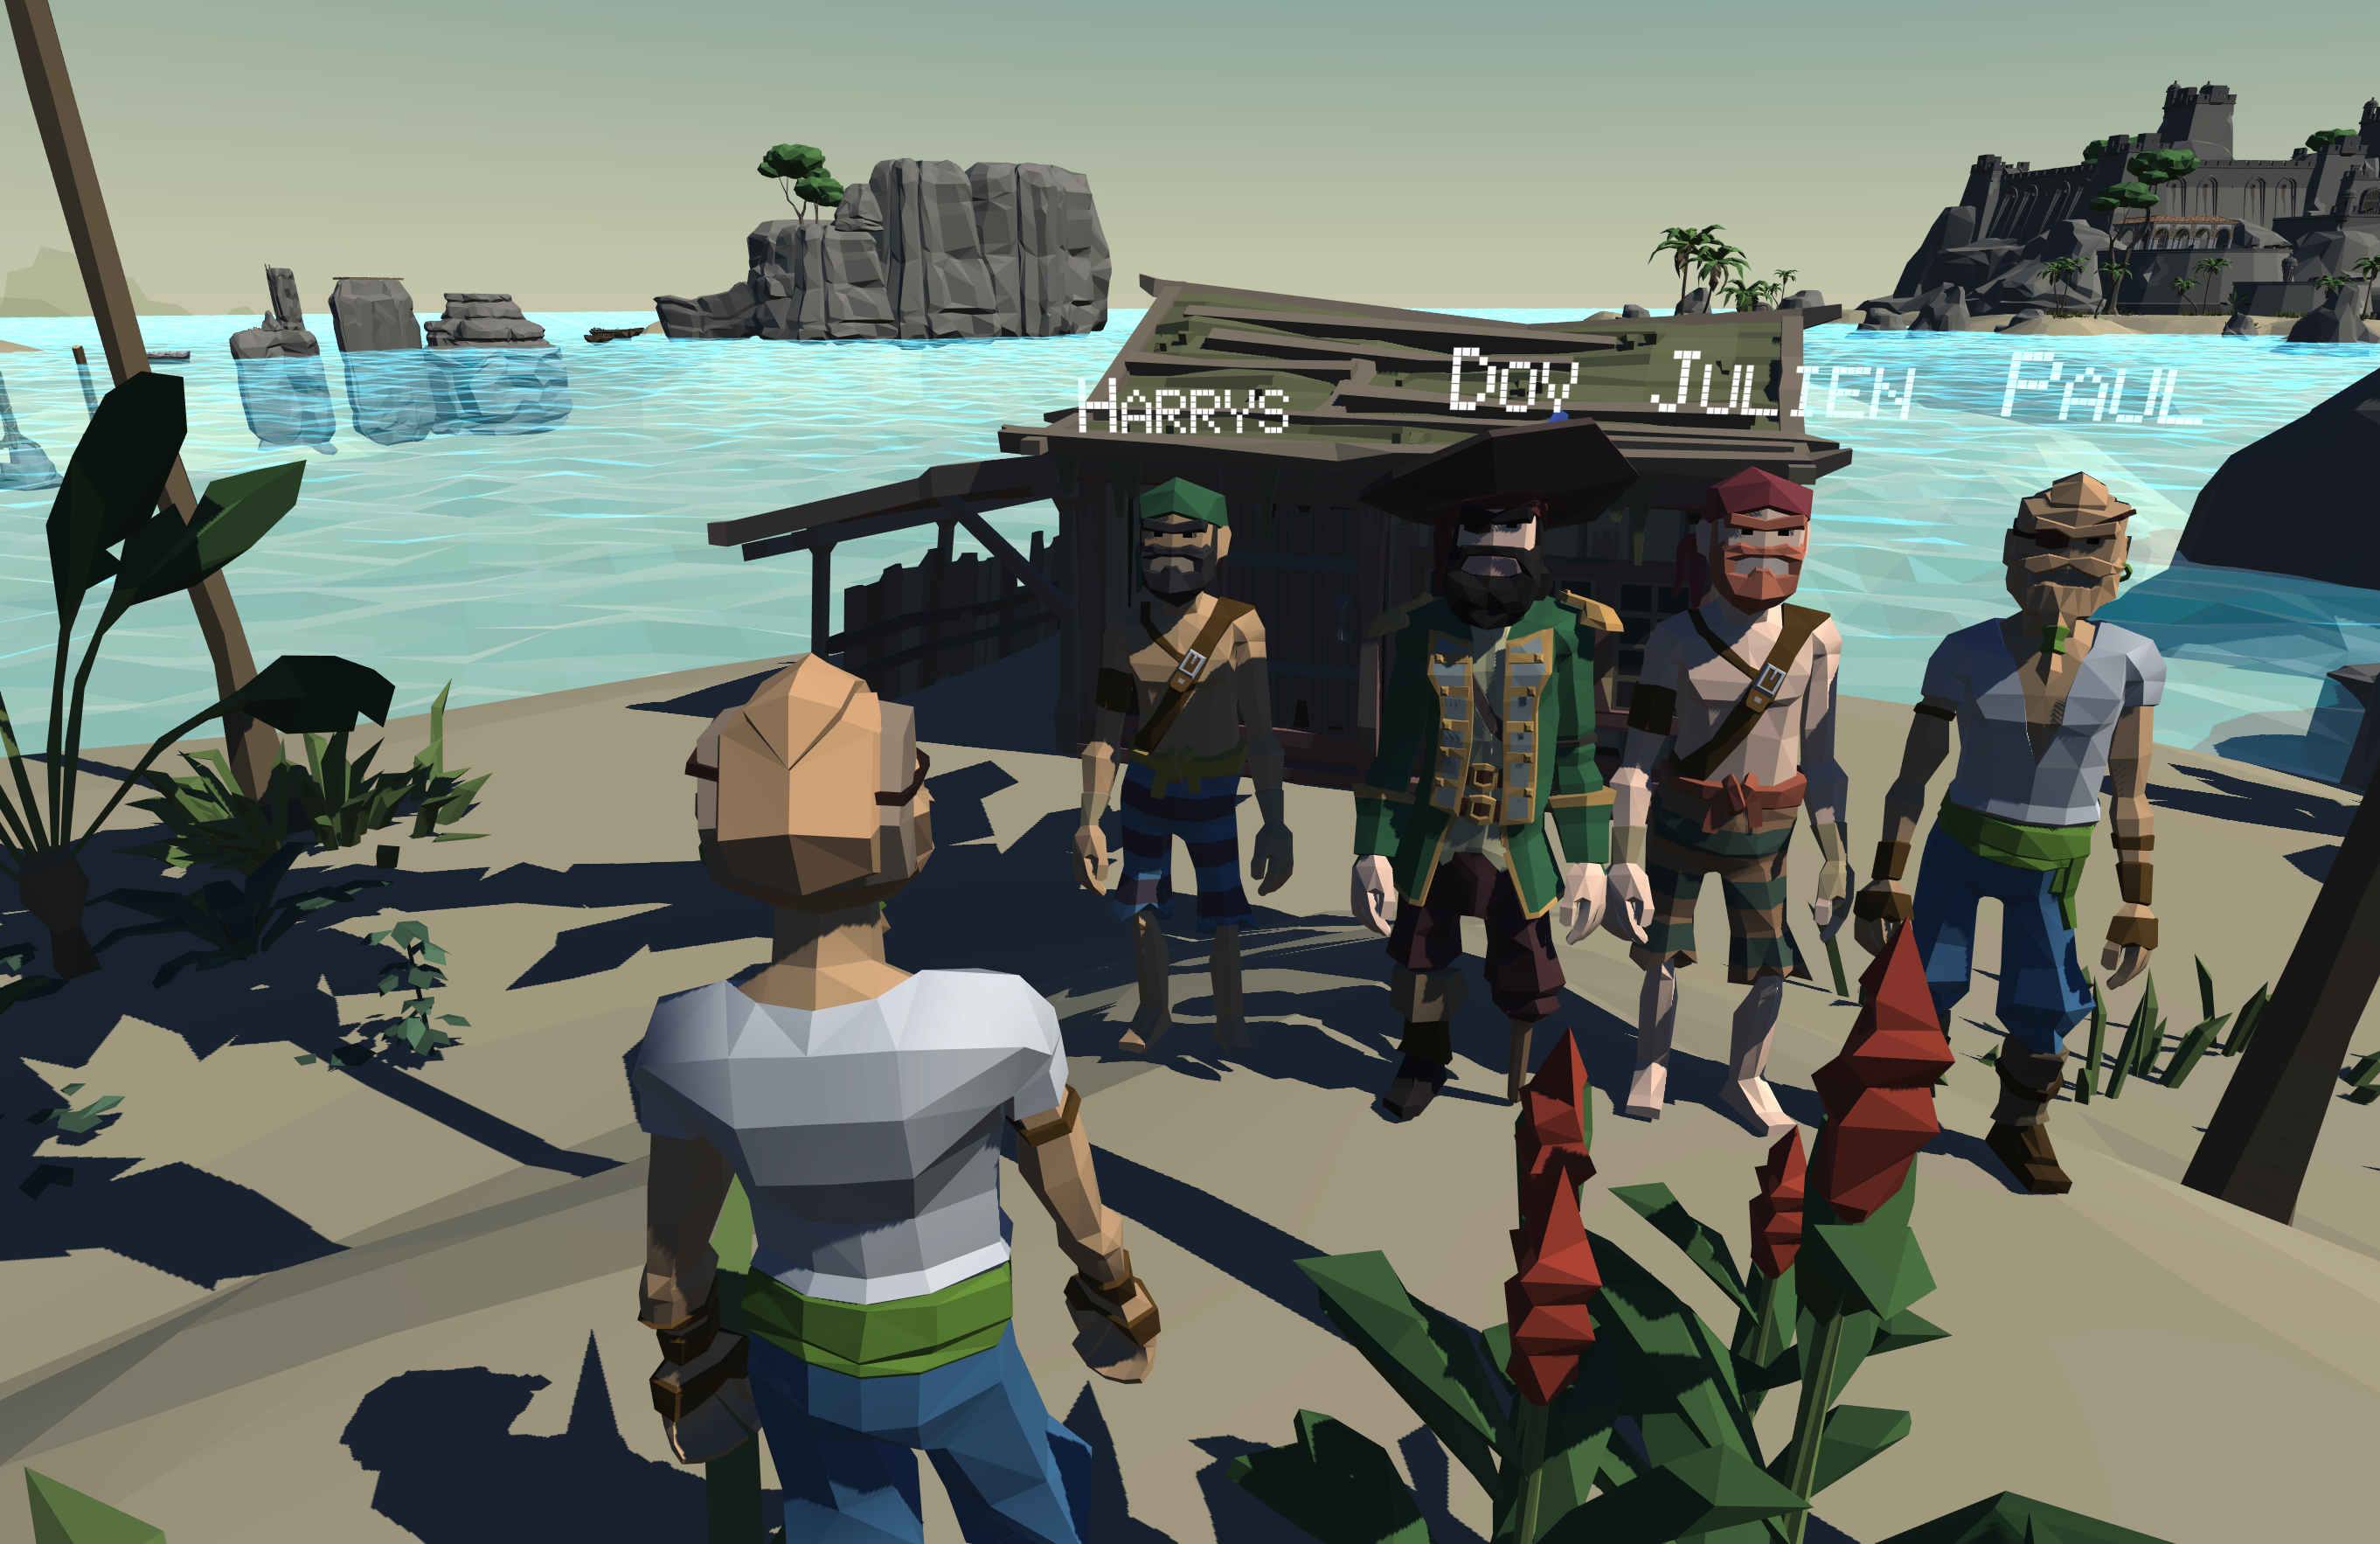
\includegraphics[scale=0.2]{in_game_lobby.png} 
                \caption{Photo de groupe en multijoueur}
            \end{figure}


        \paragraph{Transition du Lobby vers le jeu}
        
            Un système a été mis en place permettant le passage de la scène de lobby vers la scène de jeu.
            Ce système fonctionne a l'aide d'un timer, qui est synchronisé entre tout les joueurs, y compris ceux
            rejoignant le lobby après son lancement. La synchronisation se fait grâce à une fonctionnalité des salles Photon
            permettant de créer des propriétés spécifiques, couplé à la propriété PhotonNetwork.Time qui
            est identique pour tout les clients d'une salle au même moment, permettant une synchronisation
            "parfaite" des timers.
            Ce timer ne se lance uniquement après que le serveur soit à moitié remplit et dure 3 minutes. Si le nombre de joueurs descend en dessous de ce seuil, le timer s'arrête. De plus, qaund le serveur
            est complet, le temps d'attente est réduit à 30 secondes.
            A la fin du timer, le Master Client charge la map de jeu, qui est synchronisé avec tout les joueurs.



    \subsubsection{Deuxième soutenance}

        \paragraph{Synchronisation du lancement de partie}
        
            Une fois la transition effectué, il est nécessaire de synchroniser l'initialisation des différents composants
            permettant le fonctionnement d'une partie. Par exemple, il faut attendre que tout les joueurs finissent de charger
            la nouvelle scène avant d'instancier les joueurs sur la carte. Pour cela, un script s'occupe d'activer les différentes phases
            du lancement de partie suivant certaines conditions. Dans le cas de l'instantiation des joueurs, le script observe une propriété
            des joueurs déterminant si ces derniers ont chargés la map. Ainsi, le script de spawn des joueurs ne débute qu'une fois que tout les joueurs
            ont indiqué avoir chargé la carte.


        \paragraph{Synchronisation des joueurs}

            Tout comme sur le lobby, les mouvements des joueurs ainsi que leurs animations sont synchronisés. Cependant,
            un deuxième élément s'ajoute à cela: l'apparition (spawn) des joueurs. Pour cela, des points d'apparitions (spawpoints)
            sont répartis sur la map. Le Master Client distribue ces points aux joueurs qui apparaîtront à l'endroit reçu. cela permet
            de faire apparaîte chaque joueur à une position unique sur la carte : un point = un joueur, pas plus. Une fois cela fait,
            il faut également synhcroniser la réapparition des joueurs, pour cela on applique le même système, en ne prenant en compte que les joueurs
            morts.


        \paragraph{Synchronisation de l'IA}

            La grande difficulté du système multijoueur est la synchronisation des PNJs. En effet, c'est une tâche important dû à la nature du jeu, 
            mais également difficile dû au grand nombre d'IA présentes sur la map.

            Tout d'abord, il faut synchroniser l'apparition des PNJs. Le Master Client instancie les personnages grâce à Photon ; ils sont donc au départ 
            placés et visibles de la même façon pour tout les joueurs.

            Tout d'abord, il faut synchroniser l'apparition des PNJs. Encore une fois, c'est le Master Client qui instancie les personnages
            grâce à Photon. Ils sont donc au départ placé de la même façon pour tout les joueurs. Il faut également synchroniser leur apparence.
            Encore une fois, cette dernière est déterminé par le Master Client puis partagé aux autres joueurs grâce à une méthode RPC.

            Mais les problèmes commencent au moment de synchroniser le mouvement des IA. Le système qui a été créé par Dov permet
            à l'IA de se déplacer sur la map, il faut maintenant que ce mouvement soit propagé de façon quasi-identique à tout les joueurs.
            Pour cela, plusieurs méthodes ont été envisagées:

            - L'utilisation de Photon Transform View, comme pour les joueurs. Ce système a vite montré ses limites, car inadapté à la synchronisation
            d'un grand nombre d'objets, fonctionant sur la base d'un envoi pseudo-continu d'informations. Ainsi de nombreux problèmes apparaissaient,
            et la synchronisation des mouvement en a souffert. 

            - Calcul de chemin client-side à partir du même point. L'idée est la suivante: le master client calcule un point, qui est la destination
            de l'IA, et la partage aux autres joueurs. Puis chaque joueur calcule le chemin pris par l'IA pour y arriver. Cela réduit considérablement la
            quantité d'information échangée, mais un autre problème se pose: le calcul de chemin pour les NavMesh Agents n'est pas déterministe. Ainsi le
            chemin calculé par chaque client à partir du même point n'est pas le même, ce qui entraîne également une désynchronisation de la position.

            - Enfin, le choix retenu est le calcul d'un chemin entier par le Master Client, qui envoie ensuite l'intégralité de ce chemin aux autres joueurs.
            Ainsi le chemin est le même pour tout le monde, mais l'envoi des points se fait de façon discrète: on envoit uniquement l'array de positions généré
            par le Master Client. Ce système permet d'avoir une synchronisation satisfaisante des déplacement et une utilisation minime de la bande passante.

            De plus, une fois le premier chemin créé et partagé aux joueurs de la salle, il est nécessaire d'activer le mouvement des PNJ de façon la plus simultanée possible.
            Le processus est le même que celui permettant de synchroniser les timers : on crée une propriété de la salle qui indique le moment exact où
            les IAs sont activés, une fonctionnalité de Photon permettant l'accés à une valeur identique sur tout les clients au même instant (PhotonNetwork.Time).


        \paragraph{Synchronisation des assassinats et des morts}

            Une dernière partie de la synchronisation inclue celle des évènement de mort, pour les joueurs ainsi
            que les IA. Pour cela, il a été décidé d'utiliser le sytème d'Event Photon. Auparavant, la synchronisation de méthodes
            passait par l'utilisation de Photon View et de RPC. Mais le système de kill/death demande une propagation plus importante
            de l'évènement, car plusieurs systèmes différents doivent y réagir. C'est là que Photon rentre en jeu.

            En effet, ce dernier permet de synchroniser le déclenchement d'évènements. Pour cela, on utilise la méthode RaiseEvent ainsi
            qu'un code représentant notre évènement. Cette action appelle la méthode callback OnEvent, dans laquel il suffit d'associer le
            code de l'évènement à une méthode. Ainsi, à la mort d'un joueur, le tueur déclenche l'évènement mort en indiquant l'identité du
            joueur tué. Chaque joueur reçoit cet évènement et peut déterminer, par exemple, si le joueur mort est lui-même, ou bien si un
            autre joueur a tué sa cible... En bref, chaque client prend une décision en fonction de l'information reçue.
            Les détails du système de morts sont dans la partie gameplay.

            Une dernière partie de la synchronisation inclue celle des évènement de mort, pour les joueurs ainsi
            que les IA. Pour cela, il a été décidé d'utiliser le sytème d'Event Photon. Auparavant, la synchronisation de méthodes
            passait par l'utilisation de Photon View et de RPC. Mais le système de kill/death demande une propagation plus importante
            de l'évènement, car plusieurs systèmes différents doivent y réagir. C'est la que Photon rentre en jeu.

            En effet, ce dernier permet de synchroniser le déclenchement d'évènement. Pour cela, on utilise la méthode RaiseEvent ainsi
            qu'un code représentant notre évènement. Cette action appelle la méthode callback OnEvent, dans laquel il suffit d'associer le
            code de l'évènement à une méthode. Ainsi, à la mort d'un joueur, le tueur déclenche l'évènement mort en indiquant l'identité du
            joueur tué. Chaque joueur reçoit cette évènement et peut déterminer, par exemple, si le joueur mort est lui-même, ou bien si un
            autre joueur a tué sa cible... En bref, chaque client prend une décision en fonction de l'information reçu
            Les détails du système de morts sont dans la partie gameplay.


        \paragraph{Synchronisation du déroulé de partie}

            De la même manière, un système d'event a été mis en place permettant de synchroniser les différentes étapes du jeu, 
            avec une période de synchronisation des IA en début de partie, différentes manches et enfin une phase de fin avec les stats.


        \paragraph{Chat Photon}

        Enfin, un chat a été implémenté grâce à une librairie de Photon. Ce chat permet aux joueurs 
        d'une salle de communiquer entre eux, dans le lobby et en jeu.

        \begin{figure}[hbt!]
            \centering
            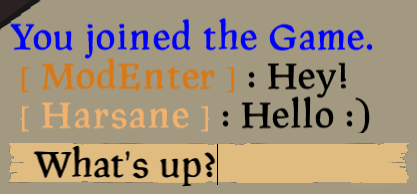
\includegraphics[scale=1]{chat.png}
            \caption{Démonstration du chat Photon}
        \end{figure}


    \subsubsection{Dernière soutenance}

        \paragraph{Synchronisation des animations de mort}
			
			Les animations de mort, créés par Dov, fonctionnent à présent en multijoueur. Un meurtre est maintenant très visible et peu discret!
			Le tueur et sa victime en particuliers profitent d'un point de vue privilégié sur cette animation avec une cinématique dynamique à l'aide de Cinémachine.
			De plus l'assassin obtient une immunité temporaire le temps de commettre l'acte, mais ce répit n'est que temporaire...
			
		\paragraph{Synchronisation des zones de discussion}
			
			Encore une fois, le travail de Dov est maintenant fonctionnel sur les serveurs Photon! Il est donc possible pour les joueurs de "camoufler" leur présence dans ces zones.
			Il est même possible d'avoir plusieurs joueur parlant dans la même zone! Bien sûr, les assassinats sont toujours possible sur les PNJs et joueurs dans la zone, rester immobile
			n'est donc pas forcément la meilleure idée dans toutes les situations.
			
	    \paragraph{Amélioration du système de synchronisation des PNJ}
			
			Le système de synchronisation passe d'une horloge globale qui dirige le départ de chaque PNJ à un système d' "horloge interne", qui permet de démarrer/arrêter
			chaque personnage de façon individuel. Cela est particulièrement utile pour l'implémentation des zones de discussion, mais aussi pour organiser un "départ différé" de l'IA.
			En effet, synchroniser simultanément plus d'une centaine de personnages n'est pas une très bonne idée. Ainsi, il est maintenant possible de le faire sur une plage de temps
			plus large, ce qui permet d'éviter les problèmes de bande passante et certaines limitations de Photon.
		
		\paragraph{Implémentation des pouvoirs en multijoueur}
		
			Les pouvoirs sont maintenant présent en jeu ! les 4 pouvoirs (lancer de couteau, déguisement, vitesse, et poison) sont tous parfaitement fonctionnels et utilisable sur les PNJs
			comme sur les autres joueurs! Un menu de séléction de pouvoir a aussi été implémenté, ainsi qu'une option permettant de choisir un pouvoir au hasard et un timeout qui éxécute ce choix
			automatiquement si le joueur ne le fait pas manuellement au bout d'un certain temps.
			
		\paragraph{Implémentation de la scène de fin de jeu}
		
			Le jeu se termine maintenant de façon beaucoup plus satisfaisante avec l'implémentation en multijoueur d'une petite cinématique de fin de jeu, qui montre un classement ainsi
			que les pires joueurs de la partie! Ont été également intégrés les animations de victoire.
		
			
		
		